\chapter{Étude des structures de données}


%nombre de caractéristiques ?? de quels type 

%Regarder JDK allocation d'une boite structure


%lister toutes les possibilité - garder toutes les structures - reconstruire l'arbre.. refaire une passe sur le fichier


\section{Introduction}
L'objectif de ce document est de mener une étude sur les différentes structures de données nécessaires aux futurs algorithmes de visualisation. Les calculs de compléxité seront réalisés selon le paramètre $n$  représentant le nombre de boîtes, et $d$ est le nombre de dimensions du problème. Le nombre de boîtes réellement utilisées dans le pavage est représenté par $N$.\textbf{Vérifier pour N}


\section{Définition de la boîte}
C'est l'entité du pavage. Les accès à ses attributs sont donc cruciaux. On rappelle qu'une boîte est définie de la manière suivante : 
\begin{itemize}
\item 
  Un identifiant : Une \verb+String+ respectant un format précis (c.f 1.1 du document de spécifications).
\item
  Une liste de coordonnées. Une liste de type \verb+Interval+.
\item
  Une liste des caractéristiques, dans l'ordre et selon les types définis en entête
\end{itemize}
Ces données seront régulièrement requises durant les algorithmes nécessaires à la visualisation. Il est donc important que leurs accès soient rapides, voir direct. Pour le cas de l'identifiant, s'agissant d'une simple \verb+String+ le problème de la structure à utiliser ne se pose pas. Pour la liste des coordonnées en revanche, il s'agit d'une séquence finie de données. Plusieurs possibilités sont alors envisageables : 

\begin{itemize}
\item
  Un tableau : L'accès à une coordonnée serait direct. Les opérations d'ajout et de suppression sont revanches coûteuses. Or il est peu probable que ce type d'opération intervienne. 
\item
  Une liste : Si l'accès à une coordonnée ne serait pas direct, les opérations d'ajouts de de suppressions sont en temps constant. Ces caractéristiques ne conviennent pas à notre problème.
\item
  Une hashmap : Coûteuse si la fonction de hashage n'est pas appropriée, la HashMap propose cependant un accès direct. Cependant même pour un petit nombre d'éléments, son occupation mémoire peut être conséquente. 
\item
  Une TreeMap \cite{TreeMap}. Implémentation de base des arbres rouges noirs, cette map a la particularité de posséder des clefs triées. Ainsi les complexités de plusieurs opérations telle que l'accès en $\log{n}$. Dans le cas d'un grand nombre de valeurs à stocker, il est plus performant de construire la TreeMap à partir d'une HashMap.

\end{itemize}

%La création d'une boîte a alors une complexité en $O(d)$. De plus l'accès aux différents attributs de la boîte (identifiant, liste des coordonnées) sera en $O(1)$.

\subsection{Variables et identifiants}
Il est nécessaire de faire le lien de manière efficace entre le nom d'une variable, et sa place dans la structure. En effet comment savoir par exemple que la valeur \verb+x+ se trouve à la position 4 dans la structure de données.
\begin{itemize}
\item
  Selon le document de spécifications, les variables sont données dans un ordre précis, donné dans l'entête du fichier d'entrée. On peut alors utiliser une map «gobale» renseignant la position de chaque variable. Si cette méthode permet de gagner de l'espace mémoire au sein d'une boîte, le nombre d'accès à cette map risque d'être élevé.
\item
  Utiliser une TreeMap (la clef étant le nom de la variable).
\end{itemize} 

\subsection{Généricité des caractéristiques}
Un problème majeur apparaît pour l'instanciation des boîtes. On rappelle qu'une caractéristique a plusieurs types (\verb+String+, \verb+Number+ ou \verb+Interval+). Plusieurs solutions sont envisageables : 
\begin{itemize}
\item 
  Chaque boîte possède trois maps pour ces trois types de caractéristiques. Cette solution à l'inconvénient d'être coûteuse si par exemple une boîte ne possède que des caractéristiques de type \verb+String+ et aucunes de types \verb+Number+ ou \verb+Interval+. 
\item
  Une map unique contenant des \verb+String+ stocke les différentes caractéristiques de la boîte. On aura casté les attributs \verb+Number+ ou \verb+Interval+ en \verb+String+.
\item 
Trois tableaux (un pour chaque type) au sein d'une boîte. Trois maps (une pour chaque type) «générales» au niveau du pavage. La clef d'une map est l'id de la caractéristique et la valeur de la map son indice dans le tableau concret. La boîte retrouve l'indice au sein d'une caractéristique son tableau .

\end{itemize}


\section{Pavage}
L'outil de visualisation peut charger un fichier entrée de manière dynamique ou non. Nous nous plaçons ici dans le cadre où cette option de chargement dynamique n'est pas activée. \\ L'outil va lire donc de manière  séquentielle chaque ligne du fichier d'entrée. Le cahier de spécification exige fréquement un listing de boîtes. Par exemple pour afficher la listres des boîtes concernées par un filtre. La structure du pavage doit être en mesure de répondre de manière efficaces à des requêtes d'un séquence d'un nombre de  boîtes selon un ordre particulier. La structure du pavage doit être aussi en mesure de répondre efficacement à la structure  de visualisation graphique (cf \textbf{lien dym vers QuadTree}). On peut d'emblée envisager plusieurs stratégie pour le stockage du pavage :

\begin{itemize}
\item
  Le fichier d'entrée est lu une unique fois. Les méthodes  de structures dans laquelle les boîtes sont stockées sont suffisament performante pour répondre à toutes les spécifications. On peut alors se poser la question si il faut 
  \begin{itemize}
  \item
    Insérer les boîtes dans la structure puis la trier plus tard.
  \item
    Utiliser un tris par insertion.
  \end{itemize}
\item
  Il est possible que refaire des «passes» sur le fichier d'entrée soit une solution. Dans les cas où les opérations de tris et/ou de recherches seraient trop coûteuse pour la structure du pavage (par exemple lors d'une demande de listing de certaines boîtes). On aurait une complexité en pire cas en $O(n)$. 
  % Le création de structure de  données peut alors se faire de différentes  manières : 
  % Chaque boîte est crée de manière séquentielle selon l'ordre du fichier puis stockée dans la structure de donnée. Le trie de la structure aura lieu plus tard ., 
\end{itemize}
\subsection{Stockage du pavage}
Le nombre potentiellement très grand de boîtes élimine d'emblée la possibilité de choisir une HashMap. En effet même si la fonction de hashage est judicieusement choisie, l'occupation mémoire requise serait bien trop importante. Les listes ne sont pas  appropriées ici. Une complexité en $n²$ pour un accès à une boîte n'est pas raisonnable. Les arbres ont l'atout de pouvoir stocker et manipuler un grand nombre de d'entités. Les arbres de recherches sont des arborescences ordonnées permettant un accès en $\log(n)$. Dans le cas où la structure serait triée au fur et à mesure de sa construction. Les arbres de recherche proposent de bonnes performances. Nous developperons pourquoi à travers des cas d'exemples dans les prochains paragraphes : 



\paragraph{Arbre binaire}
Par exemple l'utilisation d'un arbre binaire de recherche pour la création de n boîtes aurait une complexité de $n²$ en pire cas. En effet il s'agit du cas où les boîtes arriveraient triées selon l'ordre inverse de celui que l'on souhaite. Il faudrait alors effecter $(p-1)$ comparaisons, pour chaque boîte :  $\sum_{p=2}^{n}(p-1)$  Soit $O(n)=\frac{1}{2}n²-\frac{1}{2}n$. Cependant dans le meilleur des cas cette opération a une complexité en $n\log{n}$.
La création d'un pavage composé de n boîtes à d dimensions aurait alors une complexité égale à: $(n*d)*n\log(n)$ $\triangle$

\begin{figure}[htbp]
  \centering
  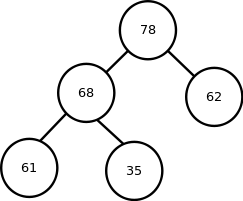
\includegraphics[scale=0.60]{img/binTree}
  \caption{a-b tree}
  \label{fig:dnuages}
\end{figure}

%http://www.enseignement.polytechnique.fr/profs/informatique/Luc.Maranget/421/poly/arbre-bin.html
\clearpage
\paragraph{Arbres a-b}
Il s'agit d'un arbre de recherche avec les propriétés suivantes :
\begin{itemize}
\item
  $a\leq2$ et $b\leq 2a−1$ deux entiers
\item
  La racine a au moins 2 fils (sauf si l'arbre ne possède qu'un noeud) et au plus b fils,
\item 
  Les feuilles sont de même profondeur,
\item
  les autres nœuds internes ont au moins a et au plus b fils
\end{itemize}

\begin{figure}[htbp]
  \centering
  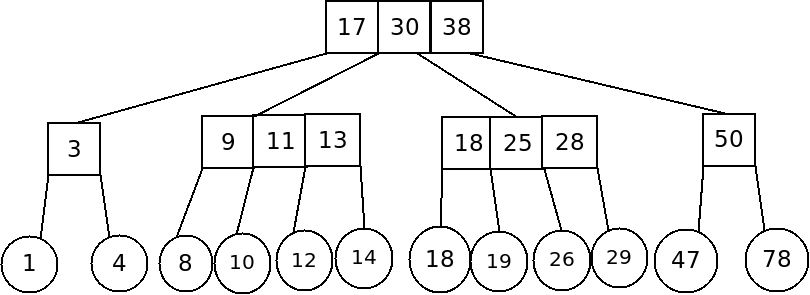
\includegraphics[scale=0.40]{img/abtree}
  \caption{a-b tree}
  \label{fig:dnuages}
\end{figure}


L'avantage des arbres a-b est que leurs hauteurs sont sont comprises entres les valeurs suivantes : $ \dfrac{\log{n}}{\log{b}}   \leq h  < 1 + \dfrac{\log{n/2}}{\log{a}}$. Ainsi les opération d'insertions ne serait plus en $n\log{n}$ mais en $\log{n}$.

La création d'un pavage composé de n boîtes à d dimensions aurait alors une complexité égale à: $(n\times d)\times\log(n)$ $\triangle$


